\clearpage
\section{CHANGE OF VARIABLE}
If $g:[a,b]\to \F{R}$ is continuously differentiable and $f: \F{R}\to \F{R}$
is continuous, then, as is well know 
\begin{align*}
    \int_{g(a)}^{g(b)} f = \int_a^b (f\circ g)\cdot g'
\end{align*}

The proof is very simple: if $F' = f$, then $(F\circ g)' = (f\circ g)\cdot g'$;
thus the left side is $F(g(b)) - F(g(a))$, while the right side is $F\circ g(b) - F\circ g(a)
= F(g(b)) - F(g(a))$.

We leave it to the reader to show that if $g$ is 1-1, then the above formula can be wriiten
\begin{align*}
    \int_{g((a,b))} f = \int_{(a,b)} f\circ g\cdot |g'|
\end{align*} 

(Consider separately the cases where $g$ is increasing and where
$g$ is decreasing.) The generalization of this formula to higher
dimensions is by no means so trivial.


\begin{theorem}
    Let $A\subset \F{R}^n$ be an open set and $g:A\to \F{R}^n$ a 1-1, continuously differentiable
    function such that $\det g'(x)\neq 0$ for all $x\in A$. If $f:g(A)\to \F{R}$ is Integrable, then
    \begin{align*}
        \int_{g(A)} f = \int_A (f\circ g)|\det g'|
    \end{align*} 
\end{theorem}

\begin{proof}
1. Suppose there is an admissible cover $\C{O}$ for $A$ such that
for each $U \in \C{O}$ and any integrable $f$ we have
\begin{align*}
    \int_{g(U)} f = \int_U (f\circ g)|\det g'|
\end{align*}
Then the theorem is true for all of $A$. (Since $g$ is automatically 1-1 in an open set 
around each point, it is not surprising that this is the only part of the proof using the fact
that $g$ is 1-1 on all of $A$.)

\textit{Proof of (1)}. The collection of all $g(U)$ is an open cover of
$g(A)$. Let $\Phi$ be a partition of unity subordinate to this cover.
If $\varphi = 0$ outside of $g(U)$, then, since $g$ is 1-1, we have 
$(\varphi\cdot f)\circ g =0$ outside of $U$. Therefore the equation 
\begin{align*}
    \int_{{g}({U})}{\varphi}\cdot{f}=\int_{{U}}\left[({\varphi}\cdot{f})\circ{g}]\right|\det g'|
\end{align*}

can be written 
\begin{align*}
    \int_{{g}({A})}{\varphi}\cdot{f}=\int_{{A}}\left[({\varphi}\cdot{f})\circ{g}]\right|\det g'|
\end{align*}

Hence 
\begin{align*}
    \int_{g(A)}^{}{f} 
    & = \sum_{\varphi\in\Phi}^{}{\int_{g(A)} \varphi\cdot f} 
        = \sum_{\varphi\in\Phi}^{}{\int_A [(\varphi\cdot f)\circ g] |\det g'|} \\
    & = \sum_{\varphi\in\Phi}^{}{\int_A (\varphi\circ g)(f \circ g) |\det g'|}\\
    & = \int_A (f\circ g) |\det g'|
\end{align*}

\textit{Remark.} The theorem also follows from the assumption that
\begin{align*}
    \int_Vf = \int_{g^{-1}(V)} (f\circ g) |\det g'|
\end{align*}

for $V$ in some admissible cover of $g(A)$. This follows from (1)
applied to $g^{-1}$.

2. It suffices to prove the theorem for the function f = 1.\par 
\textit{Proof of (2)}. If the theorem holds for $f = 1$, it holds for
constant functions. Let $V$ be a rectangle in $g(A)$ and $P$ a 
partition of $V$. For each subrectangle $S$ of $P$ let $f_s$ be the 
constant function $m_S(J)$. Then
\begin{align*}
    L(f, P) 
    & = \sum_{S}^{}{m_S(f)\cdot v(S)} = \sum_{S }^{}{\int_{\R{int}\; S} f_S} \\
    & = \sum_{S }^{}{\int_{g^{-1}(\R{int}\; S)} (f_S\circ g)|\det g'|}
        \le \sum_{S}^{}{\int_{g^{-1}(\R{int}\; S)} (f\circ g)|\det g'|} \\
    & \le \int_{g^{-1}(V)} (f\circ g)|\det g'|
\end{align*}

Since $\int_V f$ is the least upper bound of all $L(f,P)$, this proves that 
$\int_V f \le \int_{g^{-1}(V)} (f\circ g)|\det g'|$. A similar argument, letting 
$f_S = M_S(f)$, shows that $\int_V f \ge \int_{g^{-1}(V)} (f\circ g)|\det g'|$. The result 
now from the above Remark.

3. If the theorem is true for $g:A\to \F{R}^n$ and for $h:B\to \F{R}^n$, where 
$G(A)\subset B$, then it is true for $h\circ g:A\to \F{R}^n$.

\textit{Proof of (3)}. 
\begin{align*}
    \int_{h\circ g(A)} f 
    & = \int_{h(g(A))} f 
        = \int_{g(A)} (f\circ h)|\det h'| \\
    & = \int_A [(f\circ h)\circ g] \cdot [|\det (h)'|\circ g]\cdot |\det g'| \\
    & = \int_A f\circ (h\circ g) \cdot |\det (h\circ g)'|
\end{align*}

4. The theorem is true if g is a linear transformation.\par
Proof of (4). By (1) and (2) it suffices to show for any open
rectangle $U$ that
\begin{align*}
    \int_{g(U)} 1 = \int_U |\det g'|
\end{align*}

This is Problem 3-35.

Observations (3) and (4) together show that we may assume
for any particular $a \in A$ that $g'(a)$ is the identity matrix: in
fact, if Tis the linear transformation $Dg(a)$, then $(T^{-1}\circ g)'(a)=I$;
since the theorem is true for $T$, if it is true for $T^{-1}\circ g$ it will
be true for $g$.

We are now prepared to give the proof, which preceeds by
induction on $n$. The remarks before the statement of the
theorem, together with (1) and (2), prove the case $n = 1$.
Assuming the theorem in dimension $n-1$, we prove it in
dimension $n$. For each $a\in A$ we need only find an open set
$U$ with $a\in U \subset A$ for which the theorem is true.
Moreover we may assume that $g'(a)=I$. 

Define $h:A\to \F{R}^n$ by $h(x) = (g^1(x), \cdots, g^{n-1}(x), x^n)$. Then $h'(a)=I$. Hence 
in some open $U'$ with $a\in U'\subset A$, the function $h$ is 1-1 and $\det h'(x)\neq 0$. We 
can thus define $k: h(U')\to \F{R}^n$ by $k(x)=(x^1, \cdots, x^{n-1}, g^n(h^{-1}(x)))$ and 
$g=k\circ h$. We have thus expressed $g$ as the composition of two maps, each of which changes
fewer than $n$ coordinates (Figure \ref{Fig 3-3}).

\clearpage
\begin{figure}[!htb]
    \centering
    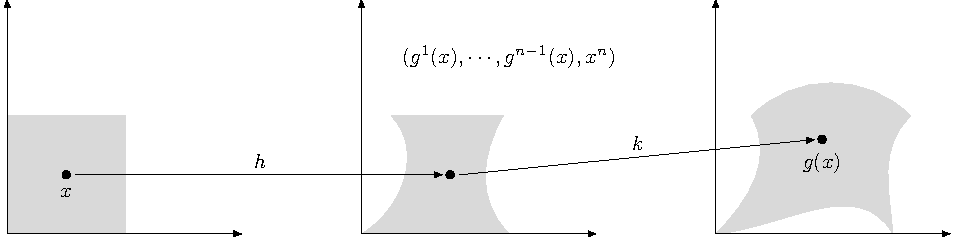
\includegraphics[width=1.4\linewidth, angle=90]{./pics/Fig3-3.pdf}
    \caption{}
    \label{Fig 3-3}
\end{figure}

\clearpage
We must attend to a few details to ensure that $k$ is a function
of the proper sort. Since
\begin{align*}
    (g^n\circ h^{-1})'(h(a)) = (g^n)'(a) \cdot [h'(a)]^{-1} = (g^n)'(a)
\end{align*}

we have $D_n(g^n\circ h^{-1})(h(a)) = D_ng^n(a) = 1$, so that $k'(h(a))=I$. Thus 
in some open set $V$ with $h(a)\in V\subset h(U')$, the function $k$ is 1-1 and 
$\det k'(x)\neq 0$. Letting $U=k^{-1}(V)$ we now have $g=k\circ h$, where $h:U\to \F{R}^n$
and $k:V\to \F{R}^n$ and $h(U)\subset V$. By (3) it suffice to prove the theorem for $h$
and $k$. We give the proof for $h$; the proof for $k$ is similar and easier.

Let $W\subset U$ be a rectangle of the form $D\times [a_n,b_n]$, where $D$ is a rectangle in 
$\F{R}^{n-1}$. By Fubini's theorem 
\begin{align*}
    \int_{h(W)} 1 = 
    \int_{[a_n, b_n]} \left(\int_{h(D\times \{x^n\})} 1\;\dd x^1\cdots \dd x^{n-1}\right)\;\dd x^n
\end{align*}

Let $h_{x^n}: D\to \F{R}^{n-1}$ be defined by 
\begin{align*}
    h_{x^n}(x^1, \cdots, x^{n-1}) = g^1(x^1, \cdots, x^n),\cdots, g^{n-1}(x^1, \cdots, x^n)
\end{align*}

Then each $h_{x^n}$ is clearly 1-1 and 
\begin{align*}
    \det (h_{x^n})'(x^1, \cdots, x^{n-1}) 
    = 
    \det h'(x^1, \cdots, x^n) \neq 0
\end{align*}

Moreover 
\begin{align*}
    \int_{h(D\times \{x^n\})} 1\;\dd x^1\cdots \dd x^{n-1} 
    = 
    \int_{h_{x^n}(D)} 1\;\dd x^1\cdots \dd x^{n-1}
\end{align*}

Applying the theorem in the case $n-1$ therefore gives
\begin{align*}
    \int_{h(W)} 1 
    & = \int_{[a_n, b_n]} \left(\int_{h_{x^n}(D)} 1\;\dd x^1\cdots \dd x^{n-1}\right)\;\dd x^n \\
    & = \int_{[a_n, b_n]} \left(\int_{D} |\det (h_{x^n})'(x^1, \cdots, x^{n-1}) \;\dd x^1\cdots \dd x^{n-1}\right)\;\dd x^n \\
    & = \int_{[a_n, b_n]}^{}\left(\int_D |\det h'(x^1, \cdots, x^n)|\;\dd x^1\cdots \dd x^{n-1}\right)\dd x^n \\
    & = \int_W |\det h'|
\end{align*}

The condition $\det g'(x)\neq 0$ may be eliminlated from the hypotheses of Theorem 3-13 
by using the following theorem, which often plays an unexpected role.
\end{proof}

\begin{theorem}[Scard's Theorem]
    Let $g:A\to \F{R}^n$ be continuously differentiable, where $A\subset \F{R}^n$ is open, and 
    let $B=\{x\in A:\det g'(x)=0\}$ . Then $g(B)$ has measure 0.
    \label{test}
\end{theorem}

\begin{proof}
    Let $U\subset A$ be a closed rectangle such that all sides
of $U$ have length $l$, say. Let $\varepsilon > 0$. If $N$ is sufficiently large
and $U$ is divided into $N^n$ rectangles, with sides of length $l/N$,
then for each of these rectangles $S$, if $x\in S$ we have
\begin{align*}
    |Dg(x)(y-x) - g(y) - g(x)| 
    < \varepsilon |x-y|
    \le \varepsilon \sqrt{n}(l/N) 
\end{align*}

for all $y\in S$. If $S$ intersects $B$ we can choose $x\in S\cap B$;
since $\det g'(x)=0$, the set $\{Dg(x)(y-x):y\in S\}$ lies in an $(n-1)$-dimensional 
subspace $V$ of $\F{R}^n$. Therefore the set $\{g(y)-g(x):y\in S\}$ lies within $\varepsilon\sqrt{n}l/N$
of $V$, so that $\{g(y):y\in S\}$ lies within $\varepsilon\sqrt{n}l/N$ of the $(n-1)$-plane 
$V+g(x)$. On the other hand, by Lemma 2-10 there is a number $M$ such that
\begin{align*}
    |g(x) - g(y)| < M|x-y| \le M\sqrt{n} (l/N)
\end{align*}

Thus, if $S$ intersects $B$, the set $\{g(y):y\in S\}$ is contained in a cylinder whose 
height is $<2\varepsilon \sqrt{n}(l/N)$ and whose base is an $(n-1)$-dimensional sphere
of radius $<M\sqrt{n}(l/N)$. This cylinder has volume $<C(l/N)^n\varepsilon$ for some constant $C$.
There are at most $N^n$ such rectangles $S$, so $g(U\cap B)$ lies in a set of volume $<C(l/N)^n\cdot 
\varepsilon \cdot N^n = Cl^n\cdot \varepsilon$. Since this is true for all $\varepsilon > 0$,the set 
$g(U\cap B)$ has measure 0. Since (Problem 3-13) we can cover all of $A$ with a sequence of such 
rectangles $U$, the desired result follows from Theorem 3-4. 
\end{proof}


Theorem 3-14 is actually only the easy part of Sard's Theorem. The statement and proof of the 
deeper result will be found in \cite{sternberg1964lectures}, page 47.

\begin{problems}
    \problem{
        Use Theorem 3-14 to prove Theorem 3-13 without the assumption $\det g'(x) \neq 0$.
    }
    \problem{
        If $g:\F{R}^n\to \F{R}^n$ and $\det g'(x)\neq 0$, prove that in some open set 
        containing $x$ we can write $g=T\circ g_n\circ \cdots \circ g_1$, where $g_i$
        is of the form $g_i(x)=(x^1, \cdots, f_i(x), \cdots, x^n)$, and $T'$ is a linear
        transformation. Show that we can write $g=g_n\circ \cdots \circ g_1$ if and only if 
        $g'(x)$ is diagonal matrix.
    }
    \problem{
        Define $f:\{r:r>0\}\times (0, 2\pi)\to \F{R}^2$ by $f(r, \theta) = (r\cos\theta, r\sin\theta)$.
        \begin{enumerate}[label=(\alph*)]
            \item Show that $f$ is 1-1, compute $f'(r, \theta)$, and show that $\det f'(r, \theta)\neq 0$
                for all $(r, \theta)$. Show that $f(\{r:r>0\}\times (0, 2\pi))$ is the set $A$ of Problem 
                2-23.
            \item If $P=f^{-1}$, show that $P(x,y) = (r(x,y), \theta(x,y))$, where 
                \begin{align*}
                    & r(x,y) = \sqrt{x^2+y^2}, 
                    & \theta(x,y) = \left\{\begin{aligned}
                        & \arctan y/x && x>0, y>0 \\
                        & \pi + \arctan y/x && x<0 \\
                        & 2\pi + \arctan y/x && x>0, y<0\\
                        & \pi/2 && x=0, y>0 \\
                        & 3\pi/2 && x=0, y<0
                    \end{aligned}\right.
                \end{align*}
                (Here $\arctan$ denotes the inverse of the function $\tan: (-\pi/2, \pi/2)\to \F{R})$
                Find $P'(x,y)$. The function $P$ is called the \textbf{polar coordinate system} on $A$.
            \item Let $C\subset A$ be the region between the circles of radii $r_1$ and
                $r_2$ and the half-lines through 0 which make angles of $\theta_1$ and $\theta_2$ with
                the $x$-axis. If $h:C\to \F{R}$ is integrable and $h(x,y) = g(r(x,y), \theta(x,y))$,
                show that 
                \begin{align*}
                    \int_C h = \int_{r_1}^{r_2} rg(r,\theta) \;\dd \theta\dd r
                \end{align*}
                If $B_r = \{(x,y):x^2+y^2\le r^2\}$, show that 
                \begin{align*}
                    \int_{B_r} h = \int_0^r \int_0^{2\pi} rg(r, \theta)\;\dd\theta\dd r
                \end{align*}
            \item If $C_r = [-r, r]\times [-r, r]$, show that 
                \begin{align*}
                    \int_{B_r}\R{e}^{-(x^2+y^2)}\;\dd x\dd y = \pi (1-\R{e}^{-r^2})
                \end{align*}
                and 
                \begin{align*}
                    \int_{C_r}\R{e}^{-(x^2+y^2)}\;\dd x\dd y = \left(\int_{-r}^r \R{e}^{-x^2}\;\dd x\right)^2
                \end{align*}
            \item Prove that 
                \begin{align*}
                    \lim_{r\to \infty} \int_{B_r} \R{e}^{-(x^2+y^2)} \;\dd x\dd y 
                    = 
                    \lim_{r\to\infty}{\int_{C_r} \R{e}^{-(x^2+y^2)}}\;\dd x\dd y
                \end{align*}
                and conclude that
                \begin{align*}
                    \int_{-\infty}^\infty \R{e}^{-x^2}\;\dd x = \sqrt{\pi}
                \end{align*}
        \end{enumerate}
    }
\end{problems}


\vspace*{12em}
\begin{center}
    ``A mathematician is one to whom that is as obvious as that twice
two makes four is to you. Liouville was a mathematician.''\par 
\hfill --- LORD KELVIN
\end{center}